\subsection{All About the G5RV Antenna: What You Need to Know!}

Which of the following describes a G5RV antenna?
\begin{tcolorbox}[colback=gray!10, colframe=black, title=E9C09]
\begin{enumerate}[label=\Alph*.]
    \item \textbf{A wire antenna center-fed through a specific length of open-wire line connected to a balun and coaxial feed line}
    \item A multi-band trap antenna
    \item A phased array antenna consisting of multiple loops
    \item A wide band dipole using shorted coaxial cable for the radiating elements and fed with a 4:1 balun
\end{enumerate} \end{tcolorbox}

\subsubsection*{Related Concepts}

The G5RV antenna is an important design in the field of radio communication and is well-suited for amateur radio operations. Understanding this antenna involves a few key concepts:

\begin{itemize}
    \item \textbf{Antenna Types:} The G5RV is primarily categorized as a wire antenna. Its design is focused on achieving multi-band capabilities using a specific configuration of feed lines.
    \item \textbf{Feed Line:} The term 'center-fed' indicates that the antenna is fed at its center, which often leads to improved performance and radiation characteristics across the desired frequencies.
    \item \textbf{Balun:} A balun (balanced to unbalanced transformer) is employed to connect the open-wire feed line to the coaxial cable. This helps in matching the impedance of the antenna system to the feed line.
\end{itemize}

\subsubsection*{Antenna Configuration}

The G5RV antenna is typically configured as follows:

1. It consists of a wire (or wires) that can be of several lengths, often around 102 feet, which provides good performance on multiple bands, especially 20 to 10 meters.
2. The center-fed design utilizes a specific length of open-wire line (usually around 450 ohm), allowing it to be fed effectively with a balun connecting to 50 ohm coaxial cable.

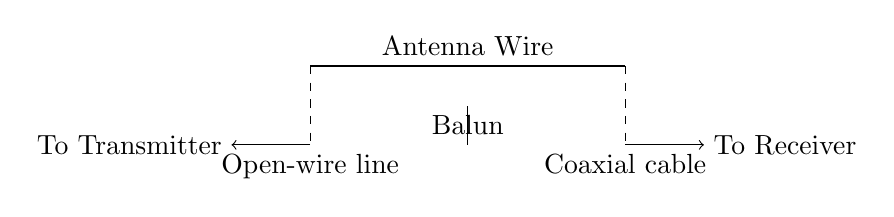
\begin{tikzpicture}
    \draw[thick] (-2,0) -- (2,0) node[midway, above] {Antenna Wire};
    \draw[dashed] (-2,0) -- (-2,-1) node[below] {Open-wire line};
    \draw[dashed] (2,0) -- (2,-1) node[below] {Coaxial cable};
    \draw[->] (-2,-1) -- (-3,-1) node[left] {To Transmitter};
    \draw[->] (2,-1) -- (3,-1) node[right] {To Receiver};
    \draw (0,-1) -- (0,-0.5) node[below] {Balun};
\end{tikzpicture}

\subsubsection*{Conclusion}

Given the options presented, the correct answer to the question is option A: A wire antenna center-fed through a specific length of open-wire line connected to a balun and coaxial feed line. This encapsulates the essential characteristics and functionalities of the G5RV antenna design, emphasizing its simplicity and versatility for amateur radio enthusiasts.
